Continuous Bag-of-Words (CBOW) un Continuous Skip-gram Model ir divas neironu tīklu modeļu arhitektūras jēdzientelpu izveidei balstoties uz teksta korpusa. CBOW modelī (konteksta distributed reprezentation jeb) apkārt esošos vārdus izmanto vidū esošā vārda paredzēšanai. Skip-gram modelī vārda vektoru izmanto konteksta paredzēšanai.

\begin{figure}[h]
	\centering
	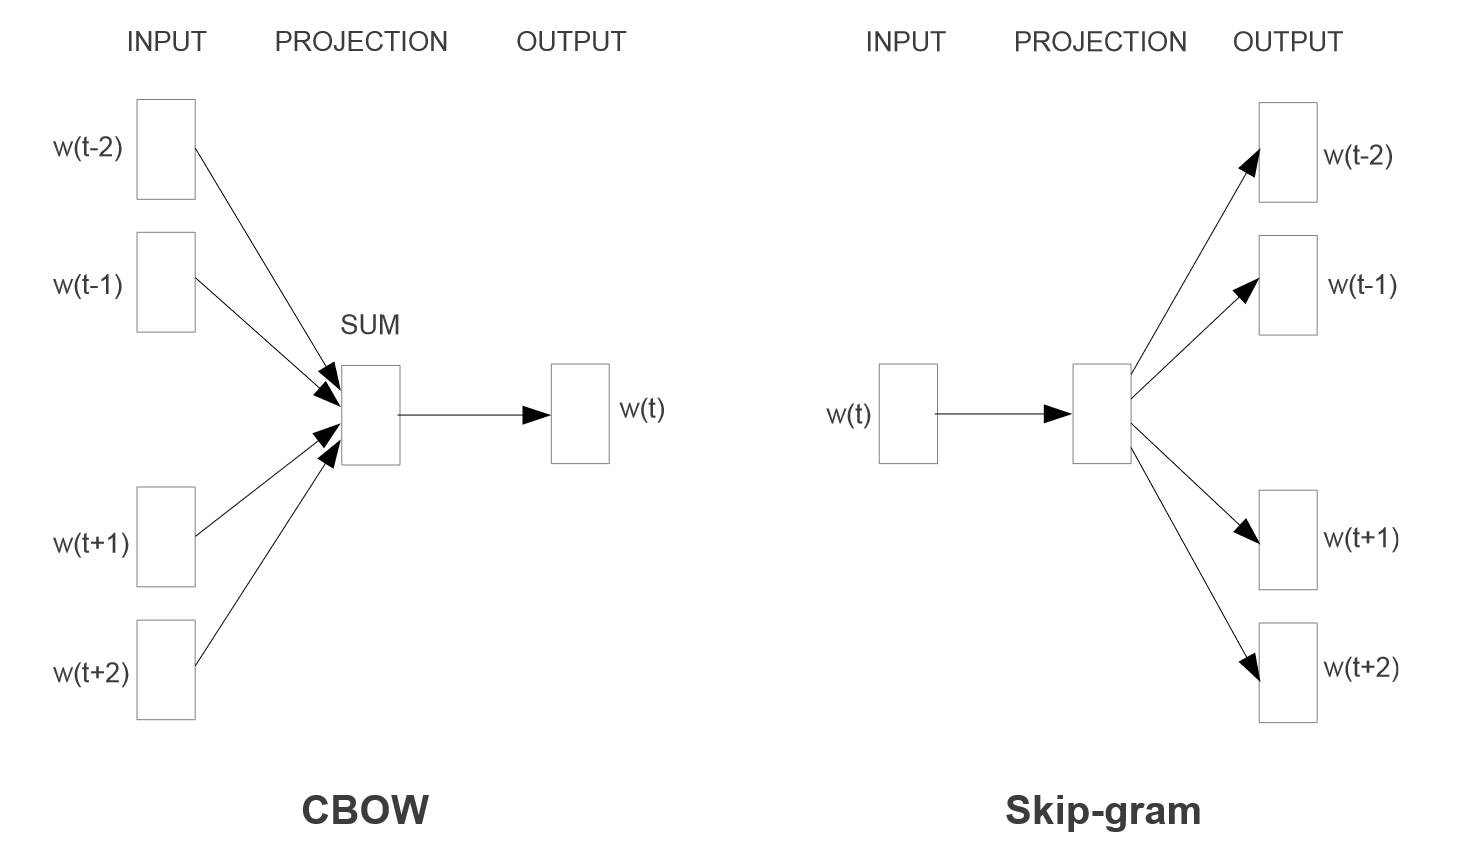
\includegraphics[width=\textwidth]{figures/word2vec-models.png}
	\caption{Vārdu vektoru piemērs, kur katra dimensija ir novērtēta ar svariem un atbilst hipotētiskai vārda nozīmes niansei \cite{word2vec2013}.}
	\label{fig:cbow-skipgram}
\end{figure}



Ideja un cosine of the angle
\url{https://en.wikipedia.org/wiki/Vector_space_model}

test
\cite{word2vec2013}.

test2 \cite{mikolov2013exploiting}.


\section{Continuous Bag-of-Words}

Bag-of-Words (BOW) apzīmē vārdu grupu nesaglabājot kārību. Vienā izlasē (bag) vārda tuvums mērķa vārdam konkrētā izlasē nav tik svarīgs, atkārtojot procesu uz korpusa no konteksta tāpat tiks sīkāk (granulētāk) izšķirti svari tuvākajiem vārdiem, piemēram, Rīga un Latvija būs tuvumā 1000 reizes biežāk nekā Rīga un sniegs.
% \url{https://en.wikipedia.org/wiki/Bag-of-words_model}

CBOW (Continuous Bag-of-Words) metodē neironu tīkls mēģina uzminēt esošo (vidējo) vārdu no n iepriekšējiem un n nākošajiem vārdiem. Procesu atkārtojot, vārdiem, kas bieži parādās vienā kontekstā, būs līdzīgi vektori. Pēc distributional hypothesis vārdi, kas atrodas līdzīgos kontekstos, ir ar līdzīgu nozīmi \cite{word2vec2013}.


Šo arhitektūru mēs saucam par BOW modeli, jo vārdu secība vēsturē neietekmē projekciju.

Tāpat kā BOW modelis, CBOW vārdu secība neietekmē projekciju. 

Mēs šo modeli raksturojam vēl vairāk kā CBOW, jo atšķirībā no standarta BOW modeļa tas izmanto nepārtrauktu konteksta dalītu attēlojumu.

\section{Continuous Skip-gram Model}


Koncepts ir uztrennēt neironu tīklu ar slēpto slāni (hidden layer) un izmantot slēptā slāņa svarus kā vārdu vektorus.
Mērķis/koncepts ir iegūt slēptā slāņa svarus, kas patiesībā arī ir vārdu vektori.

Uzdevums ir no input vārda (vārdu pa vārdam) paredzēt apkārt esošos vārdus. Kaimiņu vārdu skaits - loga lielums (window size) ir hiperparametrs

[attēls ar modeli, caption dimensijas]
Dimensijas
Input vector 1xV — where V is the number of words in the vocabulary
The single hidden layer will have dimension VxE, where E is the size of the word embedding and is a hyper-parameter.
The output from the hidden layer would be of the dimension 1xE, which we will feed into an softmax layer.
The dimensions of the output layer will be 1xV, where each value in the vector will be the probability score of the target word at that position.

[piemērs]


\cite{mccormick2016}


\section{Modeļu performance/salīdzinājums/rezultāti}

Metožu priekšrocība ir tajā, ka nav nepieciešama anotēta treniņu datu kopa, trennēšanai izmanto lielu tekstu korpusu (internetā ir daudz lielu teksta korpusu).


"Skip-gram works well with a small amount of the training data, represents well even rare words or phrases.
CBOW several times faster to train than the skip-gram, slightly better accuracy for the frequent words." 
\url{https://groups.google.com/g/word2vec-toolkit/c/NLvYXU99cAM/m/E5ld8LcDxlAJ}
